% This is file JFM2esam.tex
% first release v1.0, 20th October 1996
%       release v1.01, 29th October 1996
%       release v1.1, 25th June 1997
%       release v2.0, 27th July 2004
%       release v3.0, 16th July 2014
%   (based on JFMsampl.tex v1.3 for LaTeX2.09)
% Copyright (C) 1996, 1997, 2014 Cambridge University Press

\documentclass{jfm}
\usepackage{graphicx}
\usepackage{epstopdf, epsfig}

\newcommand{\mrd}{\mathrm{d}}
\newtheorem{lemma}{Lemma}
\newtheorem{corollary}{Corollary}

\shorttitle{Guidelines for authors}
\shortauthor{A. N. Other, H.-C. Smith and J. Q. Public}

\title{Viscous control of shallow elastic fracture}

\author{Alan N. Other\aff{1}
  \corresp{\email{jfm@damtp.cam.ac.uk}},
  H. - C. Smith\aff{1}
 \and J. Q.  Public\aff{2}}

\affiliation{\aff{1}Department of Chemical Engineering, University of America,
Somewhere, IN 12345, USA
\aff{2}Department of Aerospace and Mechanical Engineering, University of
Camford, Academic Street, Camford CF3 5QL, UK}

\begin{document}

\maketitle

\begin{abstract}
This paper considers the problem of a semi-infinite crack parallel to the
boundary of a half plane, with the crack filled by an incompressible viscous
fluid. 
The dynamics are driven by a bending moment applied to the arm of the crack,
and we look for travelling wave solutions. We examine two models of fracture;
fracture with a single tip, and fracture with a wet tip proceded by a region
of dry fracture.
\end{abstract}

\begin{keywords}
Authors should not enter keywords on the manuscript, as these must be chosen by the author during the online submission process and will then be added during the typesetting process (see http://journals.cambridge.org/data/\linebreak[3]relatedlink/jfm-\linebreak[3]keywords.pdf for the full list)
\end{keywords}

\section{Introduction}\label{sec:introduction}
Here we review the literature as well as describe the problem in more detail.
We have the vertical displacement $h$, the horizontal displacement $g$, the
thickness of the arm $l$, and the pressure $p$.
We look for a travelling wave solution (propagating left), with speed $c$.
 
\section{Formulation of problem}\label{sec:formulation_of_problem}
From lubrication, we expect Poiselle flow in the crack. This gives us the
flux, $q$, as 
\begin{equation}
q = - \frac{1}{12\mu}\frac{\mrd p}{\mrd x}h^3
\end{equation}
We also have the conservation equation
%
\begin{equation}
\frac{\partial q}{\partial x} + \frac{\partial h}{\partial t} = 0 
\end{equation}
Which combined gives us the equation
\begin{equation}
\frac{\mrd p}{\mrd x} = 12\mu c / h^2
\end{equation}
From the linear theory of elasticity, due to others who have studied this 
problem, we have
\begin{equation}
\setlength{\arraycolsep}{2pt}
\left[ \begin{array}{c} 
\sigma_y \\ \tau_{xy}
\end{array} \right]
= \int_0^{\infty} \mathsfbi{K}(x - \tilde{x}) 
\left[ \begin{array}{c} 
g'(\tilde{x}) \\ h'(\tilde{x})
\end{array} \right]
\mrd \tilde{x} 
\end{equation}
%
Where the integral kernel is
\begin{equation}
\setlength{\arraycolsep}{2pt}
\renewcommand{\arraystretch}{1.3}
\mathsfbi{K} = \left[
\begin{array}{ccccc}
  K_{11}  &  K_{12}  \\
K_{21} & K_{22} \\
\end{array}  \right] 
\end{equation}
Here we change into a set of dimensionless variables, and will spend the 
rest of the paper working with them.
We have a length scale $l$, a pressure scale $p^* = E/12(1-\nu^2)$, and a
time scale $t^* = 12\mu /p^*$.
From these, we can define the following dimensionless parameters,
\begin{equation}
\mathcal{M} = \frac{M}{p^* l^2}, \qquad \mathcal{C} = \frac{c}{l/t^*}
= \frac{12\mu c}{p^* l}, \qquad \mathcal{K}_I = \frac{K_I}{p^* l^{1/2}},
\qquad \mathcal{K}_{II} = \frac{K_{II}}{p^* l^{1/2}} 
\end{equation}
and variables 
\begin{equation} 
x = l\xi, \quad K_{ij} = U_{ij} /l, \quad h = \alpha l H(\xi), \quad
g = \alpha l G(\xi), \quad p = \beta p^* \Pi(\xi)
\end{equation}
The preferred scalings to be used in this paper are $\alpha = \upi \beta /3
= \mathcal{M}$, $\lambda = \upi\mathcal{C}/3\mathcal{M}^2$, which give
\begin{equation}
\setlength{\arraycolsep}{2pt}
\left[ \begin{array}{c} 
\Pi \\ 0
\end{array} \right]
= \int_0^{\infty} \mathsfbi{U}(\xi - \tilde{\xi}) 
\left[ \begin{array}{c} 
G'(\tilde{\xi}) \\ H'(\tilde{\xi})
\end{array} \right]
\mrd \tilde{\xi}, \qquad
H^2 \frac{\mrd \Pi}{\mrd \xi} = \lambda
\end{equation}
\begin{equation}
\lim_{\xi \to \infty} H'' = 1 , \quad \lim_{\xi \to \infty} G' = \frac{1}{2}
\end{equation}
\begin{equation}
\lim_{\xi \to 0} 3\sqrt{2\pi \xi} H' = \frac{K_I}{M l^{-3/2}} \equiv \kappa_I , 
\quad
\lim_{\xi \to 0} 3\sqrt{2\pi \xi} G' = \frac{K_{II}}{M l^{-3/2}} 
\equiv \kappa_{II} , 
\end{equation}
These shall be the governing equations for the rest of this paper.
\section{Numerical scheme}\label{sec:numerical_scheme}
\subsection{Single Tip}
We discretize the problem by taking n points $\boldsymbol{\xi} = (\xi_1, \dots
,\xi_n)$ at which we measure $H'$, $G'$, and $n-1$ intermediate points 
$\boldsymbol{\zeta} = (\zeta_1, \dots , \zeta_{n-1})$ at which to measure
$\Pi$, so that $\xi_1 < \zeta_1 < \dots < \zeta_{n-1} < \xi_n$. We take
$\xi_1 = 0$, where the crack tip is situated.
Linear interpolation of $G'$,$H'$ would work poorly near the crack tip, since
both functions are singular there. However, both $\sqrt{\xi}G'(\xi)$, and
$\sqrt{\xi}H'(\xi)$ are regular functions, so we work with these instead,
near the tip.
\subsection{Double Tip}
Here we mention details specific to the problem with both a fluid
and a dry tip. Perhaps details of the $\sin^2$ spacing or the interpolation
to $K_I=0$ should be mentioned here.
 
\section{Results}\label{sec:Results}
Here we put the majority of the graphs which show the results of the numerics.
\section{Discussion}
This is where we discuss the figures, possibly include more figures, and draw
the results and conclusions of this paper.
\subsection{Figures}

\begin{figure}
  \centerline{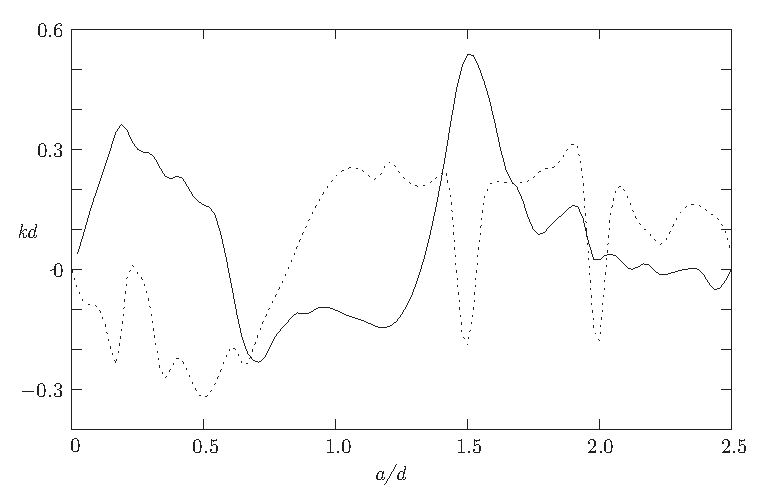
\includegraphics{trapped}}% Images in 100% size
  \caption{Trapped-mode wavenumbers, $kd$, plotted against $a/d$ for
    three ellipses:\protect\\
    ---$\!$---,
    $b/a=1$; $\cdots$\,$\cdots$, $b/a=1.5$.}
\label{fig:ka}
\end{figure}

\begin{figure}
  \centerline{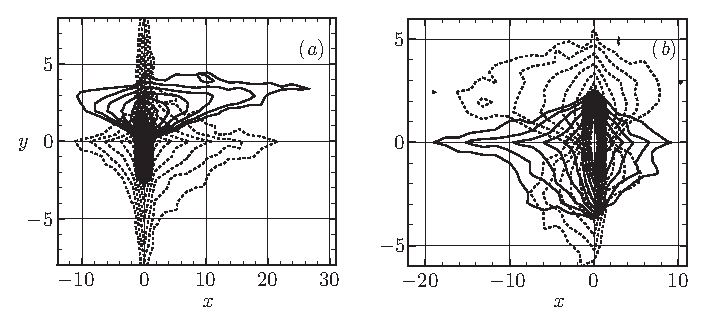
\includegraphics{modes}}
  \caption{The features of the four possible modes corresponding to
  (\textit{a}) periodic\protect\\ and (\textit{b}) half-periodic solutions.}
\label{fig:kd}
\end{figure}

\subsection{Tables}
Tables, however small, must be numbered sequentially in the order in which they are mentioned in the text. The word \textit {table} is only capitalized at the start of a sentence. See table \ref{tab:kd} for an example.

\begin{table}
  \begin{center}
\def~{\hphantom{0}}
  \begin{tabular}{lccc}
      $a/d$  & $M=4$   &   $M=8$ & Callan \etal \\[3pt]
       0.1   & 1.56905 & ~~1.56~ & 1.56904\\
       0.3   & 1.50484 & ~~1.504 & 1.50484\\
       0.55  & 1.39128 & ~~1.391 & 1.39131\\
       0.7   & 1.32281 & ~10.322 & 1.32288\\
       0.913 & 1.34479 & 100.351 & 1.35185\\
  \end{tabular}
  \caption{Values of $kd$ at which trapped modes occur when $\rho(\theta)=a$}
  \label{tab:kd}
  \end{center}
\end{table}

\subsection{Mathematical notation}
\subsubsection{Setting variables, functions, vectors, matrices etc}
{\bf Italic font} should be used for denoting variables, with multiple-letter symbols avoided except in the case of dimensionless numbers such as $\Rey$, $\Pran$ and $\Pen$ (Reynolds, Prandtl, and P\'eclet numbers respectively, which are defined as \verb}\Rey}, \verb}\Pran} and {\verb}\Pen} in the template).\\
{\bf Upright Roman font} (or upright Greek where appropriate) should be used for:\\
Operators: sin, log, d, $\Delta$, e etc.\\
Constants: i ($\sqrt{-1}$), $\upi$ (defined as \verb}\upi}), etc.\\
Functions: $\Ai$, $\Bi$ (Airy functions, defined as \verb}\Ai} and \verb}\Bi}), $\Real$ (real part, defined as \verb}\Real}), $\Imag$ (imaginary part, defined as \verb}\Imag}), etc.\\
Physical units: cm, s, etc\\
Abbreviations: c.c. (complex conjugate), h.o.t. (higher-order terms), DNS, etc.\\
{\bf Bold italic font} (or bold sloping Greek) should be used for:\\
Vectors (with the centred dot for a scalar product also in bold): $\boldsymbol{i \cdot j}$\\
{\bf Bold sloping sans serif font}, defined by the \verb}\mathsfbi} macro, should be used for:\\
Tensors and matrices: $\mathsfbi{D}$ \\
{\bf Script font} (for example $\mathcal{G}$, $\mathcal{R}$) can be used as an alternative to italic when the same letter denotes a different quantity (use \verb}\mathcal} in \LaTeX)\\
The product symbol ($\times$) should only be used to denote multiplication where an equation is broken over more than one line, to denote a cross product, or between numbers (the $\cdot$ symbol should not be used, except to denote a scalar product specifically).\\ 

\subsubsection{Other symbols}
A centred point should be used only for the scalar product of vectors.
Large numbers that are not scientific powers should not include commas, but have the
form 1600 or 16 000 or 160 000.
Use \textit{O} to denote `of the order of', not the \LaTeX\ $\mathcal{O}$.

\section{Citations and references}
All papers included in the References section must be cited in the article, and vice versa. Citations should be included as, for example ``It has been shown \citep{Rogallo81} that...'' (using the {\verb}\citep} command, part of the natbib package) ``recent work by \citet{Dennis85}...'' (using {\verb}\citet}).
The natbib package can be used to generate citation variations, as shown below.\\
\verb#\citet[pp. 2-4]{Hwang70}#:\\
\citet[pp. 2-4]{Hwang70} \\
\verb#\citep[p. 6]{Worster92}#:\\
\citep[p. 6]{Worster92}\\
\verb#\citep[see][]{Koch83, Lee71, Linton92}#:\\
\citep[see][]{Koch83, Lee71, Linton92}\\
\verb#\citep[see][p. 18]{Martin80}#:\\
\citep[see][p. 18]{Martin80}\\
\verb#\citep{Brownell04,Brownell07,Ursell50,Wijngaarden68,Miller91}#:\\
\citep{Brownell04,Brownell07,Ursell50,Wijngaarden68,Miller91}\\
The References section can either be built from individual \verb#\bibitem# commands, or can be built using BibTex. The BibTex files used to generate the references in this document can be found in the zip file at http://journals.cambridge.org/\linebreak[3]data/\linebreak[3]relatedlink/\linebreak[3]jfm-ifc.zip.\\
Where there are up to ten authors, all authors' names should be given in the reference list. Where there are more than ten authors, only the first name should appear, followed by et al.\\

Acknowledgements should be included at the end of the paper, before the References section or any appendicies, and should be a separate paragraph without a heading. Several anonymous individuals are thanked for contributions to these instructions.

\appendix
\section{}\label{appA}
This appendix contains sample equations in the JFM style. Please refer to the {\LaTeX} source file for examples of how to display such equations in your manuscript.

\begin{equation}
  (\nabla^2+k^2)G_s=(\nabla^2+k^2)G_a=0
  \label{Helm}
\end{equation}

\begin{equation}
  \bnabla\bcdot\boldsymbol{v} = 0,\quad \nabla^{2}P=
    \bnabla\bcdot(\boldsymbol{v}\times \boldsymbol{w}).
\end{equation}

\begin{equation}
  G_s,G_a\sim 1 / (2\upi)\ln r
  \quad \mbox{as\ }\quad r\equiv|P-Q|\rightarrow 0,
  \label{singular}
\end{equation}

\begin{equation}
\left. \begin{array}{ll}  
\displaystyle\frac{\p G_s}{\p y}=0
  \quad \mbox{on\ }\quad y=0,\\[8pt]
\displaystyle  G_a=0
  \quad \mbox{on\ }\quad y=0,
 \end{array}\right\}
  \label{symbc}
\end{equation}


\begin{equation}
  -\frac{1}{2\upi} \int_0^{\infty} \gamma^{-1}[\mathrm exp(-k\gamma|y-\eta|)
   + \mathrm exp(-k\gamma(2d-y-\eta))] \cos k(x-\xi)t\:\mathrm{d} t,
   \qquad 0<y,\quad \eta<d,
\end{equation}

\begin{equation}
  \gamma(t) = \left\{
    \begin{array}{ll}
      -\mathrm{i}(1-t^2)^{1/2}, & t\le 1 \\[2pt]
      (t^2-1)^{1/2},         & t>1.
    \end{array} \right.
\end{equation}

\[
  -\frac{1}{2\upi}
   \pvi B(t)\frac{\cosh k\gamma(d-y)}{\gamma\sinh k\gamma d}
   \cos k(x-\xi)t\:\mathrm{d} t
\]

\begin{equation}
  G = -\frac{1}{4}\mathrm{i} (H_0(kr)+H_0(kr_1))
    - \frac{1}{\upi} \pvi\frac{\mathrm{e}^{-\kgd}}%
    {\gamma\sinh\kgd} \cosh k\gamma(d-y) \cosh k\gamma(d-\eta)
\end{equation}

Note that when equations are included in definitions, it may be suitable to render them in line, rather than in the equation environment: $\boldsymbol{n}_q=(-y^{\prime}(\theta),
x^{\prime}(\theta))/w(\theta)$.
Now $G_a=\squart Y_0(kr)+\Gat$ where
$r=\{[x(\theta)-x(\psi)]^2 + [y(\theta)-y(\psi)]^2\}^{1/2}$ and $\Gat$ is
regular as $kr\ttz$. However, any fractions displayed like this, other than $\thalf$ or $\squart$, must be written on the line, and not stacked (ie 1/3).
 
\begin{eqnarray}
  \ndq\left(\frac{1}{4} Y_0(kr)\right) & \sim &
    \frac{1}{4\upi w^3(\theta)}
    [x^{\prime\prime}(\theta)y^{\prime}(\theta)-
    y^{\prime\prime}(\theta)x^{\prime}(\theta)] \nonumber\\
  & = & \frac{1}{4\upi w^3(\theta)}
    [\rho^{\prime}(\theta)\rho^{\prime\prime}(\theta)
    - \rho^2(\theta)-2\rho^{\prime 2}(\theta)]
    \quad \mbox{as\ }\quad kr\ttz . \label{inteqpt}
\end{eqnarray}

\begin{equation}
  \frac{1}{2}\phi_i = \frac{\upi}{M} \sumjm\phi_j K_{ij}^a w_j,
  \qquad i=1,\,\ldots,\,M,
\end{equation}
where
\begin{equation}
  K_{ij}^a = \left\{
    \begin{array}{ll}
      \p G_a(\theta_i,\theta_j)/\p n_q, & i\neq j \\[2pt]
      \p\Gat(\theta_i,\theta_i)/\p n_q
      + [\rho_i^{\prime}\rho_i^{\prime\prime}-\rho_i^2-2\rho_i^{\prime 2}]
      / 4\upi w_i^3, & i=j.
  \end{array} \right.
\end{equation}


\refstepcounter{equation}
$$
  \rho_l = \lim_{\zeta \rightarrow Z^-_l(x)} \rho(x,\zeta), \quad
  \rho_{u} = \lim_{\zeta \rightarrow Z^{+}_u(x)} \rho(x,\zeta)
  \eqno{(\theequation{\mathit{a},\mathit{b}})}\label{eq35}
$$

\begin{equation}
  (\rho(x,\zeta),\phi_{\zeta\zeta}(x,\zeta))=(\rho_0,N_0)
  \quad \mbox{for}\quad Z_l(x) < \zeta < Z_u(x).
\end{equation}


\begin{subeqnarray}
  \tau_{ij} & = &
    (\overline{\overline{u}_i \overline{u}_j}
    - \overline{u}_i\overline{u}_j)
    + (\overline{\overline{u}_iu^{SGS}_j
    + u^{SGS}_i\overline{u}_j})
    + \overline{u^{SGS}_iu^{SGS}_j},\\[3pt]
  \tau^\theta_j & = &
    (\overline{\overline{u}_j\overline{\theta}}
    - \overline{u}_j \overline{\theta})
    + (\overline{\overline{u}_j\theta^{SGS}
    + u^{SGS}_j \overline{\theta}})
    + \overline{u^{SGS}_j\theta^{SGS}}.
\end{subeqnarray}

\begin{equation}
\setlength{\arraycolsep}{0pt}
\renewcommand{\arraystretch}{1.3}
\slsQ_C = \left[
\begin{array}{ccccc}
  -\omega^{-2}V'_w  &  -(\alpha^t\omega)^{-1}  &  0  &  0  &  0  \\
  \displaystyle
  \frac{\beta}{\alpha\omega^2}V'_w  &  0  &  0  &  0  &  \mathrm{i}\omega^{-1} \\
  \mathrm{i}\omega^{-1}  &  0  &  0  &  0  &  0  \\
  \displaystyle
  \mathrm{i} R^{-1}_{\delta}(\alpha^t+\omega^{-1}V''_w)  &  0
    & -(\mathrm{i}\alpha^tR_\delta)^{-1}  &  0  &  0  \\
  \displaystyle
  \frac{\mathrm{i}\beta}{\alpha\omega}R^{-1}_\delta V''_w  &  0  &  0
    &  0  & 0 \\
  (\mathrm{i}\alpha^t)^{-1}V'_w  &  (3R^{-1}_{\delta}+c^t(\mathrm{i}\alpha^t)^{-1})
    &  0  &  -(\alpha^t)^{-2}R^{-1}_{\delta}  &  0  \\
\end{array}  \right] .
\label{defQc}
\end{equation}

\begin{equation}
\etb^t = \skew2\hat{\etb}^t \exp [\mathrm{i} (\alpha^tx^t_1-\omega t)],
\end{equation}
where $\skew2\hat{\etb}^t=\boldsymbol{b}\exp (\mathrm{i}\gamma x^t_3)$. 
\begin{equation}
\mbox{Det}[\rho\omega^2\delta_{ps}-C^t_{pqrs}k^t_qk^t_r]=0,
\end{equation}

\begin{equation}
 \langle k^t_1,k^t_2,k^t_3\rangle = \langle
\alpha^t,0,\gamma\rangle  
\end{equation}

\begin{equation}
\boldsymbol{f}(\theta,\psi) = (g(\psi)\cos \theta,g(\psi) \sin \theta,f(\psi)).
\label{eq41}
\end{equation}

\begin{eqnarray}
f(\psi_1) = \frac{3b}{\upi[2(a+b \cos \psi_1)]^{{3}/{2}}}
  \int^{2\upi}_0 \frac{(\sin \psi_1 - \sin \psi)(a+b \cos \psi)^{1/2}}%
  {[1 - \cos (\psi_1 - \psi)](2+\alpha)^{1/2}}\mathrm{d}x,
\label{eq42}
\end{eqnarray}
\begin{eqnarray}
g(\psi_1) & = & \frac{3}{\upi[2(a+b \cos \psi_1)]^{{3}/{2}}}
  \int^{2\upi}_0 \left(\frac{a+b \cos \psi}{2+\alpha}\right)^{1/2}
  \left\{ \astrut f(\psi)[(\cos \psi_1 - b \beta_1)S + \beta_1P]
  \right. \nonumber\\
&& \mbox{}\times \frac{\sin \psi_1 - \sin \psi}{1-\cos(\psi_1 - \psi)}
  + g(\psi) \left[\left(2+\alpha - \frac{(\sin \psi_1 - \sin \psi)^2}
  {1- \cos (\psi - \psi_1)} - b^2 \gamma \right) S \right.\nonumber\\
&& \left.\left.\mbox{} + \left( b^2 \cos \psi_1\gamma -
  \frac{a}{b}\alpha \right) F(\frac{1}{2}\upi, \delta) - (2+\alpha)
  \cos\psi_1 E(\frac{1}{2}\upi, \delta)\right] \astrut\right\} \mathrm{d} \psi,
\label{eq43}
\end{eqnarray}
\begin{equation}
\alpha = \alpha(\psi,\psi_1) = \frac{b^2[1-\cos(\psi-\psi_1)]}%
  {(a+b\cos\psi) (a+b\cos\psi_1)},
  \quad
  \beta - \beta(\psi,\psi_1) = \frac{1-\cos(\psi-\psi_1)}{a+b\cos\psi}.
\end{equation}


\begin{equation}
\left. \begin{array}{l}
\displaystyle
H(0) = \frac{\epsilon \overline{C}_v}{\tilde{v}^{{1}/{2}}_T
(1- \beta)},\quad H'(0) = -1+\epsilon^{{2}/{3}} \overline{C}_u
+ \epsilon \skew5\hat{C}_u'; \\[16pt]
\displaystyle
H''(0) = \frac{\epsilon u^2_{\ast}}{\tilde{v}^{{1}/{2}}
_T u^2_P},\quad H' (\infty) = 0.
\end{array} \right\}
\end{equation}

\begin{lemma}
Let $f(z)$ be a trial \citet[][pp.~231--232]{Batchelor59} function defined on $[0,1]$.  Let $\varLambda_1$ denote
the ground-state eigenvalue for $-\mathrm{d}^2g/\mathrm{d} z^2=\varLambda g$,
where $g$ must satisfy $\pm\mathrm{d} g/\mathrm{d} z+\alpha g=0$ at $z=0,1$
for some non-negative constant~$\alpha$.  Then for any $f$ that is not
identically zero we have
\begin{equation}
\frac{\displaystyle
  \alpha(f^2(0)+f^2(1)) + \int_0^1 \left(
  \frac{\mathrm{d} f}{\mathrm{d} z} \right)^2 \mathrm{d} z}%
  {\displaystyle \int_0^1 f^2\mathrm{d} z}
\ge \varLambda_1 \ge
\left( \frac{-\alpha+(\alpha^2+8\upi^2\alpha)^{1/2}}{4\upi} \right)^2.
\end{equation}
\end{lemma}

\begin{corollary}
Any non-zero trial function $f$ which satisfies the boundary condition
$f(0)=f(1)=0$ always satisfies
\begin{equation}
  \int_0^1 \left( \frac{\mathrm{d} f}{\mathrm{d} z} \right)^2 \mathrm{d} z.
\end{equation}
\end{corollary}

\bibliographystyle{jfm}
% Note the spaces between the initials
\bibliography{jfm-instructions}

\end{document}
